\documentclass[twoside]{article}
\usepackage{aistats2017}

% If your paper is accepted, change the options for the package
% aistats2015 as follows:
%
%\usepackage[accepted]{aistats2015}
%
% This option will print headings for the title of your paper and
% headings for the authors names, plus a copyright note at the end of
% the first column of the first page.

%%%%%%%%%%%%%%%%%%%%%%%%%%%%%%%%%%%%%%%%%%%%%%%%%%%%%%%%%%%%%%%%%%%%%%%%%%%%%%%%

\usepackage{amsmath}
\usepackage{amssymb}
\usepackage{amsthm}
\usepackage{mathtools}
\usepackage{graphicx}
\usepackage{rotating}
\usepackage{xcolor}
\usepackage[inline]{enumitem}

\usepackage{algorithm}
\usepackage[noend]{algpseudocode}
%\usepackage{algorithmicx}
%\usepackage{algorithm2e}

%\usepackage[authordate,bibencoding=auto,strict,backend=biber,natbib]{biblatex-chicago}
\usepackage[round]{natbib}   % omit 'round' option if you prefer square brackets
\bibliographystyle{plainnat}

\usepackage{tikz}
\usepackage{pgfplots}
\pgfplotsset{width=7cm,compat=1.8}

%%%%%%%%%%%%%%%%%%%%%%%%%%%%%%%%%%%%%%%%

\newtheorem{cor}{Corallary}
\newtheorem{theorem}{Theorem}
\newtheorem{lemma}{Lemma}
\newtheorem{assumption}{Condition}

\DeclareMathOperator*{\argmin}{arg\,min}
\DeclareMathOperator*{\argmax}{arg\,max}
\DeclareMathOperator*{\vecspan}{span}
\DeclareMathOperator*{\affspan}{aff}
\DeclareMathOperator*{\subG}{subG}
\DeclareMathOperator*{\tr}{tr}

%\newcommand{\smin}[1]{s_\text{min}({#1})}
\newcommand{\smin}{s_\text{min}}
\newcommand{\smax}{s_\text{max}}
\newcommand{\zero}{\text{\textbf{0}}}
\newcommand{\Zproj}{Z^{\textit{proj}}}
\newcommand{\Zreopt}{Z^{\textit{owa}}}
\newcommand{\nreopt}{n^{\textit{owa}}}
\newcommand{\Q}{\mathcal{Q}}
\newcommand{\Y}{\mathcal{Y}}
\newcommand{\X}{\mathcal{X}}
\newcommand{\matW}{\hat W}
\newcommand{\matV}{\hat V}
\newcommand{\W}{{\hat \Theta^{\textit{owa}}}}
\newcommand{\Wowa}{{\hat \Theta^{\textit{owa}}}}
\newcommand{\Waff}{\mathcal{\hat A}}
\newcommand{\WaffE}{{\mathcal{\hat A}_\E}}
\newcommand{\Wave}{{\mathcal{\hat W}^{ave}}}
\newcommand{\Wtave}{{\mathcal{W}^{ave,*}}}
\newcommand{\V}{\mathcal{V}}
\newcommand{\A}{\mathcal{A}}
\newcommand{\D}{\mathcal{D}}
\newcommand{\E}{\mathbb{E}}
\newcommand{\vv}{\mathbf{v}}
\newcommand{\x}{\mathbf{x}}
\newcommand{\y}{\mathbf{y}}
\newcommand{\w}{\theta}
\newcommand{\wkl}{\hat\w^{kl}}
\newcommand{\ahat}{\hat\alpha}
\newcommand{\afull}{\ahat^{\textit{full}}}
\newcommand{\wowa}{\hat\w^{owa}}
\newcommand{\wowafull}{\hat\w^{\textit{owa,full}}}
\newcommand{\wowastar}{\hat\w^{\textit{owa,*}}}
\newcommand{\wave}{\hat\w^{ave}}
\newcommand{\wtave}{\E\hat\w^{ave}}
\newcommand{\waver}{\hat\w^{ave,r}}
\newcommand{\wboot}{\hat\w^{boot}}
\newcommand{\wmle}{\hat\w^{mle}}
\newcommand{\wmler}{\hat\w^{mle,r}}
\newcommand{\wstar}{{\w^{*}}}
\newcommand{\wq}{\hat\w^{q}}
\newcommand{\wqstar}{\hat\w^{q^*}}
\newcommand{\dist}{\mathcal{D}}

\newcommand{\tbias}{t_{\text{\textit{bias}}}}
\newcommand{\tvar}{t_{\text{\textit{var}}}}

\newcommand{\I}{\mathcal I}
%\newcommand{\I^{-1}}{\I^{-1}}
\newcommand{\law}{\ensuremath{\xrightarrow{L}}}
\newcommand{\normal}[2]{\ensuremath{\mathcal{N}\left({{#1}},{{#2}}\right)}}
\newcommand{\subnormal}[1]{\ensuremath{\subG\left({{#1}}\right)}}
\newcommand{\trans}[1]{\ensuremath{{#1}^{\mathsf{T}}}}
\newcommand{\ltwo}[1]{{\lVert {#1} \rVert}}
\newcommand{\ltwobig}[1]{{\left\lVert {#1} \right\rVert}}
\newcommand{\lone}[1]{{\lVert {#1} \rVert}_1}
\newcommand{\lzero}[1]{{\lVert {#1} \rVert}_0}
\newcommand{\proj}[1]{\pi_{{#1}}}
\newcommand{\prob}[1]{\Pr\left[{#1}\right]}

\DeclarePairedDelimiterX{\infdivx}[2]{(}{)}{%
  #1\;\delimsize\|\;#2%
}
\newcommand{\kl}{\text{KL}\infdivx}

\newcommand{\ignore}[1]{}
\newcommand{\fixme}[1]{\textbf{FIXME:} {#1}}

%%%%%%%%%%%%%%%%%%%%%%%%%%%%%%%%%%%%%%%%%%%%%%%%%%%%%%%%%%%%%%%%%%%%%%%%%%%%%%%%

\begin{filecontents}{paper.bib}

@article{scikit-learn,
 title={Scikit-learn: Machine Learning in {P}ython},
 author={Pedregosa, F. and Varoquaux, G. and Gramfort, A. and Michel, V.
         and Thirion, B. and Grisel, O. and Blondel, M. and Prettenhofer, P.
         and Weiss, R. and Dubourg, V. and Vanderplas, J. and Passos, A. and
         Cournapeau, D. and Brucher, M. and Perrot, M. and Duchesnay, E.},
 journal={Journal of Machine Learning Research},
 volume={12},
 pages={2825--2830},
 year={2011}
}

@article{kddcup2012,
  author={Yanzhi Niu and Yi Wang and Gordon Sun and Aden Yue and Brian Dalessandro and Claudia Perlich and Ben Hamner},
  title = {The Tencent Dataset and KDD-Cup'12},
  howpublished = {URL \url{http://www.kddcup2012.org/c/kddcup2012-track2}},
  year = {2012}
}

@book{lehmann1999elements,
  title={Elements of large-sample theory},
  author={Lehmann, Erich Leo},
  year={1999},
  publisher={Springer Science \& Business Media}
}

@inproceedings{merugu2003privacy,
  title={Privacy-preserving distributed clustering using generative models},
  author={Merugu, Srujana and Ghosh, Joydeep},
  booktitle={Data Mining, 2003. ICDM 2003. Third IEEE International Conference on},
  pages={211--218},
  year={2003},
  organization={IEEE}
}

@article{dasgupta2003elementary,
  title={An elementary proof of a theorem of {J}ohnson and {L}indenstrauss},
  author={Dasgupta, Sanjoy and Gupta, Anupam},
  journal={Random Structures \& Algorithms},
  volume={22},
  number={1},
  pages={60--65},
  year={2003},
  publisher={Wiley Online Library}
}

@article{matouvsek2008variants,
  title={On variants of the {J}ohnson--{L}indenstrauss lemma},
  author={Matou{\v{s}}ek, Ji{\v{r}}{\'\i}},
  journal={Random Structures \& Algorithms},
  volume={33},
  number={2},
  pages={142--156},
  year={2008},
  publisher={Wiley Online Library}
}

@inproceedings{negahban2009unified,
  title={A unified framework for high-dimensional analysis of M-estimators with decomposable regularizers},
  author={Negahban, Sahand and Yu, Bin and Wainwright, Martin J and Ravikumar, Pradeep K},
  booktitle={Advances in Neural Information Processing Systems},
  pages={1348--1356},
  year={2009}
}

@inproceedings{mcdonald2009efficient,
  title={Efficient large-scale distributed training of conditional maximum entropy models},
  author={McDonald, Ryan and Mohri, Mehryar and Silberman, Nathan and Walker, Dan and Mann, Gideon S},
  booktitle={Advances in Neural Information Processing Systems},
  pages={1231--1239},
  year={2009}
}

@inproceedings{zinkevich2010parallelized,
  title={Parallelized stochastic gradient descent},
  author={Zinkevich, Martin and Weimer, Markus and Li, Lihong and Smola, Alex J},
  booktitle={Advances in neural information processing systems},
  pages={2595--2603},
  year={2010}
}

@incollection{vershynin2010introduction,
  title={Introduction to the non-asymptotic analysis of random matrices},
  author={Vershynin, Roman},
  journal={arXiv preprint arXiv:1011.3027},
  chapter=5,
  booktitle={Compressed Sensing, Theory and Applications},
  editor={Y. Eldar and G. Kutyniok},
  year={2012}
}

@article{spokoiny2012parametricestimation,
  title={Parametric estimation. Finite sample theory},
  author={Spokoiny, Vladimir},
  journal={The Annals of Statistics},
  volume={40},
  number={6},
  pages={2877--2909},
  year={2012},
  publisher={Institute of Mathematical Statistics}
}

@inproceedings{zhang2012communication,
  title={Communication-efficient algorithms for statistical optimization},
  author={Zhang, Yuchen and Wainwright, Martin J and Duchi, John C},
  booktitle={Advances in Neural Information Processing Systems},
  pages={1502--1510},
  year={2012}
}

@article{liu2012distributed,
  title={Distributed parameter estimation via pseudo-likelihood},
  author={Liu, Qiang and Ihler, Alexander},
  journal={arXiv preprint arXiv:1206.6420},
  year={2012}
}

@inproceedings{zhang2013information,
  title={Information-theoretic lower bounds for distributed statistical estimation with communication constraints},
  author={Zhang, Yuchen and Duchi, John and Jordan, Michael I and Wainwright, Martin J},
  booktitle={Advances in Neural Information Processing Systems},
  pages={2328--2336},
  year={2013}
}

@inproceedings{zhang2013divide,
  title={Divide and Conquer Kernel Ridge Regression.},
  author={Zhang, Yuchen and Duchi, John C and Wainwright, Martin J},
  booktitle={COLT},
  year={2013}
}

@inproceedings{zhang2012communication,
  title={Communication-efficient algorithms for statistical optimization},
  author={Zhang, Yuchen and Wainwright, Martin J and Duchi, John C},
  booktitle={Advances in Neural Information Processing Systems},
  pages={1502--1510},
  year={2012}
}

@article{hsu2012tail,
  title={A tail inequality for quadratic forms of subgaussian random vectors},
  author={Hsu, Daniel and Kakade, Sham M and Zhang, Tong and others},
  journal={Electron. Commun. Probab},
  volume={17},
  number={52},
  pages={1--6},
  year={2012}
}

@article{vw,
  author={Langford, John},
  title={Vowpal Wabbit open source project},
  %url={https://github.com/JohnLangford/vowpal_wabbit}
}

@article{agarwal2014reliable,
  title={A reliable effective terascale linear learning system.},
  author={Agarwal, Alekh and Chapelle, Olivier and Langford, John},
  journal={Journal of Machine Learning Research},
  volume={15},
  number={1},
  pages={1111--1133},
  year={2014}
}

@inproceedings{liu2014distributed,
  title={Distributed estimation, information loss and exponential families},
  author={Liu, Qiang and Ihler, Alexander T},
  booktitle={Advances in Neural Information Processing Systems},
  pages={1098--1106},
  year={2014}
}

@inproceedings{shamir2014fundamental,
  title = {Fundamental Limits of Online and Distributed Algorithms for Statistical Learning and Estimation},
  author = {Shamir, Ohad},
  booktitle = {Advances in Neural Information Processing Systems 27},
  pages = {163--171},
  year = {2014}
}

@article{duchi2014optimality,
  title={Optimality guarantees for distributed statistical estimation},
  author={Duchi, John C and Jordan, Michael I and Wainwright, Martin J and Zhang, Yuchen},
  journal={arXiv preprint arXiv:1405.0782},
  year={2014}
}

@inproceedings{garg2014communication,
  title={On communication cost of distributed statistical estimation and dimensionality},
  author={Garg, Ankit and Ma, Tengyu and Nguyen, Huy},
  booktitle={Advances in Neural Information Processing Systems},
  pages={2726--2734},
  year={2014}
}

@book{shalev2014understanding,
  title={Understanding machine learning: From theory to algorithms},
  author={Shalev-Shwartz, Shai and Ben-David, Shai},
  year={2014},
  publisher={Cambridge University Press}
}

@article{braverman2015communication,
  title={Communication lower bounds for statistical estimation problems via a distributed data processing inequality},
  author={Braverman, Mark and Garg, Ankit and Ma, Tengyu and Nguyen, Huy L and Woodruff, David P},
  journal={arXiv preprint arXiv:1506.07216},
  year={2015}
}

@inproceedings{sivakumar2015beyond,
  title={Beyond Sub-Gaussian Measurements: High-Dimensional Structured Estimation with Sub-Exponential Designs},
  author={Sivakumar, Vidyashankar and Banerjee, Arindam and Ravikumar, Pradeep K},
  booktitle={Advances in Neural Information Processing Systems},
  pages={2206--2214},
  year={2015}
}

@article{han2016bootstrap,
  title={Bootstrap Model Aggregation for Distributed Statistical Learning},
  author={Han, Jun and Liu, Qiang},
  journal={arXiv preprint arXiv:1607.01036},
  year={2016}
}
\end{filecontents}
\immediate\write18{bibtex paper}

%%%%%%%%%%%%%%%%%%%%%%%%%%%%%%%%%%%%%%%%%%%%%%%%%%%%%%%%%%%%%%%%%%%%%%%%%%%%%%%%

\begin{document}

% If your paper is accepted and the title of your paper is very long,
% the style will print as headings an error message. Use the following
% command to supply a shorter title of your paper so that it can be
% used as headings.
%
%\runningtitle{I use this title instead because the last one was very long}

% If your paper is accepted and the number of authors is large, the
% style will print as headings an error message. Use the following
% command to supply a shorter version of the authors names so that
% they can be used as headings (for example, use only the surnames)
%
%\runningauthor{Surname 1, Surname 2, Surname 3, ...., Surname n}

\twocolumn[

%\aistatstitle{Instructions for paper submissions to AISTATS 2015}
\aistatstitle{Communication-Efficient Distributed Maximum Likelihood Estimation with the Optimal Weigted Average}

\aistatsauthor{ Anonymous Author 1 \And Anonymous Author 2 \And Anonymous Author 3 }

\aistatsaddress{ Unknown Institution 1 \And Unknown Institution 2 \And Unknown Institution 3 } ]

%%%%%%%%%%%%%%%%%%%%%%%%%%%%%%%%%%%%%%%%%%%%%%%%%%%%%%%%%%%%%%%%%%%%%%%%%%%%%%%%

\begin{abstract}
We present a distributed algorithm for maximum likelihood estimation (MLE) with low communication complexity.
Our algorithm is an easy to implement modification of the standard averaging method.
In the averaging method, each machine in a cluster first solves the MLE problem on a subset of the data;
the resulting parameter vectors are then averaged together.
In our method, we perform a second round of optimization to find the \emph{optimal weighted average} of the parameter vectors.
This second optimization happens in a low dimensional space,
and so it adds negligible computational and communication costs.
%Given $m$ machines (each with $n$ data points of dimension $d$),
%we show that our algorithm reduces bias at a rate of $O(\frac{1-m/d}{n})$.
Whereas the averaging method reduces only the variance of the estimator,
our method reduces both the bias and the variance.
Our analysis is more general than the analysis of similar communication efficient algorithms that also reduce the bias.
Notably, we do not assume (as do all previous analyses) that the likelihood function is concave or that any quantities are bounded.
In practice,
this bias reduction makes our algorithm more robust to the choice of regularization parameter,
speeding up the model selection process.
\end{abstract}

%%%%%%%%%%%%%%%%%%%%%%%%%%%%%%%%%%%%%%%%

% one-shot distributed learning
% communication efficient
% non-interactive

%Used by Vowpal Wabbit \cite{vw,agarwal2014reliable}.

\section{INTRODUCTION}

Many modern datasets are too large to fit in the memory of a single machine,
so they must be partitioned onto many machines.
%These datasets are typically partitioned onto many machines.
%Statistical learning algorithms are then run in a distributed manner.
%There are two main strategies for these distributed algorithms.
To analyze these datasets, we need distributed algorithms.
Existing distributed algorithms can be classified as either interactive or non-interactive.
In this paper we propose an algorithm that exhibits the benefits of both types.

\emph{Interactive algorithms} require many rounds of communication between machines.
These algorithms often resemble standard iterative algorithms where each iteration is followed by a communication step.
The appeal of interactive algorithms is that they enjoy the same statistical regret bounds as standard sequential algorithms.
Unfortunately, these algorithms can be too slow in practice because communication is the main bottleneck in modern distributed architectures,
and these algorithms require many rounds of communication.

\emph{Non-interactive} algorithms require only a single round of communication.
They are significantly faster than interactive algorithms
but have worse regret bounds.
Recent work (discussed in Section \ref{sec:bounds}) has shown that no non-interactive algorithm can achieve regret bounds comparable to an interactive one.
The popular large scale learning system Vowpal Wabbit combines both types of algorithms to achieve good real world performance.
A non-interactive algorithm is run first to provide a good warm start to a subsequent interactive algorithm \citep{vw,agarwal2014reliable}.
%Synonyms for non-interactive algorithms used in the literature include \emph{one-shot distributed learning} and \emph{communication efficient learning}.

In this paper, we propose a \emph{semi-interactive} distributed algorithm called \emph{optimal weighted averaging} (OWA).
Our algorithm performs two rounds of communication,
so it is not subject to the existing regret bounds of non-interactive algorithms.
The amount of information communicated in the second round is small, however,
so our algorithm retains the speed advantages of non-interactive algorithms.
We now formally describe our problem and proposed solution.

\subsection{Problem Statement}
%\section{Problem Setting and Our Solution}

%Let $\Theta\subseteq\mathbb{R}^d$ be the parameter space,
%$\X\subseteq\mathbb{R}^d$ be the covariate space,
%and $\Y\subseteq\mathbb{R}$ be the response space.
%Let $Z\subset\X\times\Y$ be a set of $mn$ i.i.d. datapoints.
%Then the centralized Maximum Likelihood Estimator (MLE) is defined as
%\begin{equation}
%\wmle = \argmax_\w \sum_{(\x,y)\in Z} f(y-\trans\x\w)
%\end{equation}

Let $\Y\subseteq\mathbb{R}$ be the space of response variables,
$X\subseteq\mathbb{R}^d$ be the space of the covariates,
and $\Theta\subseteq\mathbb{R}^d$ be the parameter space.
We assume a linear model.
The log-likelihood of data point $(\x,y)\in\X\times\Y$ given the model's true parameter $\wstar\in\Theta$ is denoted by $f(y,\trans\x\wstar)$.
Our analysis in Section \ref{sec:anal} places very mild restrictions on $f$.
In particular, $f$ need not be concave with respect to $\w$.
%For our experiments in Section \ref{sec:exp}, however, we restrict ourselves to the likelihood for logistic regression
%\begin{equation}
%f(y,\trans\x\w) =
%\end{equation}
Let $Z\subset\X\times\Y$ be a dataset of $mn$ i.i.d. observations.
Finally, let $R : \Theta \to \mathbb{R}$ be a regularization function (typically the L1 or L2 norm)
and $\lambda\in\mathbb{R}$ be the regularization strength.
Then the maximum likelihood estimator is
\begin{equation}
%\wmle=\argmax_\w \sum_{i=1}^{nm} g(y_i-\trans\x_i\w)
\wmle=\argmax_\w \sum_{(\x,y)\in Z} f(y,\trans\x\w)
+ \lambda R(\theta)
.
\end{equation}
Assume that $Z$ has been partitioned onto $m$ machines so that each machine $i$ has dataset $Z_i$ of size $n$, and all the $Z_i$ are disjoint.
Then each machine calculates the local estimator
\begin{equation}
\wmle_i = \argmax_\w \sum_{(\x,y) \in Z_i} f(y,\trans\x\w)
+ \lambda R(\theta)
.
\end{equation}
Solving for $\wmle_i$ requires no communication with other machines.
%Our goal is to provide a function $q : \Theta^m \to \Theta$ that ``merges'' these estimates.
%The resulting merged estimate should have error as close to $\wmle$ as possible.
%A non-interactive distributed estimator merges these $\wmle_i$ into a single improved estimate.
Our goal is to merge the $\wmle_i$ into a single improved estimate.
The baseline example is the averaging estimator
\begin{equation}
\wave = \frac{1}{m}\sum_{i=1}^m \wmle_i
.
\end{equation}
This estimator is well studied, and in Section \ref{sec:anal} we compare this previous work to our own.
Here we briefly recall that the analysis of an estimator's error $\ltwo{\wstar-\wave}$ is typically decomposed into bias $\ltwo{\wstar - \E\wave}$ and variance $\ltwo{\E\wave-\wave}$ components.
The $\wave$ estimator is known to reduce the variance but not the bias.
Our goal is to design an estimator that reduces both variance and bias.

%Next, we need a function $q : \Theta^m \to \Theta$ that combines the parameter estimates from each machine.
%Define the resulting parameter estimate as
%\begin{equation}
%\wq = q(\wmle_1, \wmle_2, ..., \wmle_m)
%\end{equation}
%Let $\Q$ be the set of all functions from $\Theta^m\to\Theta$,
%and $Q$ be a subset of $\Q$.
%Our goal is to find the function
%\begin{equation}
%q^* = \argmin_{q\in Q} \ltwo{\wqstar - \wstar}
%\end{equation}

\subsection{Proposed Solution}

We propose a modification to the averaging estimator called the \emph{optimal weighted average} (OWA) that reduces both variance and bias.
OWA uses a second round of optimization to calculate the optimal linear combination of the $\wmle_i$s.
%Using these optimal weights, we reduce bias at a rate of $O(\sqrt{1-m/d})$.
This second optimization occurs over a small fraction of the dataset,
so its computational and communication overhead is negligible.

To motivate our estimator,
we first describe a simpler estimator that uses the entire dataset for the second round of optimization.
%The idea of our proposed solution is to find the best linear combination of the $\wmle_i$s using a second round of optimization.
Define the matrix $\matW : \mathbb{R}^{d\times m}$ to have $i$th column equal to $\wmle_i$.
Now consider the estimator
\begin{equation}
\wowafull = \matW \afull
,
\end{equation}
where
\begin{equation}
\label{eq:afull}
\afull = \argmax_\alpha \sum _{(\x,y)\in Z} f\left(y,\trans\x \matW \alpha \right)
+
\lambda R(\matW\alpha)
.
\end{equation}
%This is the maximum likelihood estimator when we restrict our
Notice also that $\wowafull$ is the maximum likelihood estimator when the parameter space $\Theta$ is restricted to $\W = \vecspan \{\wmle_i\}_{i=1}^m$.
In other words, the $\afull$ vector contains the optimal weights to apply to each $\wmle_i$ when averaging.
Figure \ref{fig:contour} shows graphically that no other estimator in $\W$ can have higher regularized empirical likelihood than $\wowafull$.

\begin{figure}
\hspace{-0.1in}
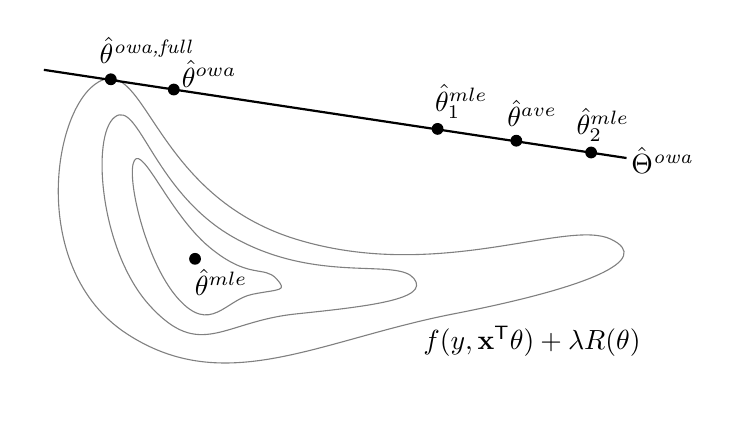
\begin{tikzpicture}
    [
    dot/.style = {minimum width=0.15cm,inner sep=0pt,line width=0pt,fill,circle,black,font=\small}
    ]
\draw[gray] plot [smooth cycle,tension=1] coordinates {(-0.5,-0.75) (-1.05,1) (-0.1,-0.1) (0.75,-0.5) (0.45,-0.7) };
\draw[gray] plot [smooth cycle,tension=1] coordinates {(-0.85,-0.85) (-1.3,1.55) (0.25,0) (2.5,-0.5) (1,-0.95)};
\draw[gray] plot [smooth cycle,tension=1] coordinates {(-1.15,-1.2) (-1.5,2) (1,0) (5,0) (3,-0.95)};

\draw[thick] (-2.2,2.15) -- (5.2,1.03);

\node[dot] (wstar) at (-0.28,-0.25) {};
\node at (0.05,-0.55) {$\wmle$};

%\node[dot] (wstarproj) at (0.1,1.8) {};
%\draw (wstar) -- (wstarproj);
%\draw (0.07,1.65) -- (0.23,1.62) -- (0.26,1.78);

%\node[dot] (wavestar) at (4,0.5) {};
%\node                 at (4.5,0.3) {$\E\wave$};
\node[dot] (wave) at (3.8,1.25) {};
\node at (4.0,1.6) {$\wave$};
\node[dot] (wave) at (2.80,1.40) {};
\node at (3.1,1.75) {$\wmle_1$};
\node[dot] (wave) at (4.75,1.10) {};
\node at (4.9,1.45) {$\wmle_2$};
%\node[dot] (wave) at (3.8,1.25) {};

\node[dot] at (-1.35,2.03) {};
\node at (-0.9,2.4) {$\wowafull$};

\node[dot] at (-0.55,1.9) {};
\node at (-0.1,2.1) {$\wowa$};

\node at (4,-1.3) {$f(y,\trans\x\w)+\lambda R(\theta)$};
\node at (5.65,1.0) {$\W$};

\end{tikzpicture}
\caption{
    Our method performs a second round of optimization to find the best parameter vector in $\W$.
    Since $\wave\in\W$, the estimator $\wowafull$ has higher empirical likelihood than $\wave$.
    Since $\W$ has low dimension, we can use relatively few data points in the second round of optimization to ensure that with high probability $\wowa$ has higher empirical likelihood than $\wave$.
}
\label{fig:contour}
\end{figure}

Calculating the weights $\afull$ directly is infeasible because it requires access to the full dataset.
Fortunately, we don't need to consider all the data points for an accurate estimator.
The parameter space $\W$ is $m$-dimensional.
So intuitively, we only need $O(m)$ data points to solve the second optimization to our desired accuracy.
%(This intuition is formalized in Section \ref{sec:anal}.)
This intuition motivates the following estimator.
Let $\Zreopt_i\subset Z_i$ be a set of $\nreopt$ data points uniformly sampled from $Z_i$ without replacement,
and let $\Zreopt$ be the union of the $\Zreopt_i$s.
Then the OWA estimator is defined as
\begin{equation}
\wowa = \matW \ahat,
\end{equation}
where
\begin{equation}
\label{eq:ahat}
\ahat = \argmax_\alpha \sum _{(\x,y)\in \Zreopt} f\left(y,\trans\x \matW \alpha \right)
+ \lambda R (\matW\alpha)
.
\end{equation}

Algorithm \ref{fig:alg2} shows the steps for efficiently computing $\wowa$.
In the first round, each machine calculates $\wmle_i$ independently and broadcasts the result to every other machine.
Since the parameter vector has $d$ dimensions and there are $m$ machines, a total of $O(md)$ bits are transmitted.
In the second round, each machine projects its local dataset $\Zreopt_i$ onto the space $\W$.
These projected data points are then transmitted to a predesignated master machine.
The projected data points each have dimension $m$, so a total of $O(m^2\nreopt)$ bits are transmitted.
The master machine now has all of the information to complete the optimization.

\begin{algorithm}[t]
\caption{Distributed calculation of $\wowa$}
\label{alg:distributed}
\begin{algorithmic}
\State Each machine $i$ independently
\State ~~~~~loads dataset $Z_i$
\State ~~~~~calculates $\wmle_i$
\State All machines broadcast $\wmle_i$ to all other machines
\State Each machine $i$ independently
\State ~~~~~constructs $\matW$
\State ~~~~~randomly selects a dataset $Z^{reopt}_i\subset Z_i$
\State ~~~~~calculates $\Zproj_i=\{(\trans\x\matW,y) : (\x,y)\in\Zreopt\}$
\State All machines broadcast $\Zproj_i$ to a master machine
\State The master calculates $\wowa$
\end{algorithmic}
\label{fig:alg2}
\end{algorithm}

\subsection{Implementation Tips}

Equations \ref{eq:afull} and \ref{eq:ahat} cannot be solved directly using off the shelf optimizers because existing optimizers do not support the non-standard regularization term $R(\matW\alpha)$.
In practice, it is sufficient to approximate this regularization by L2 regularization directly on the $\alpha$ vector:
\begin{equation}
\lambda R(\matW\alpha) \approx \lambda_2 \ltwo{\alpha}
.
\end{equation}
Intuitively, this is because even when we want the parameter vector $\w$ to be sparse (and so are regularizing by $R = $ the L1 norm), we have no reason to believe that the $\alpha$ vector should be sparse.
The desired sparsity is induced by the regularization when solving for $\wmle_i$s and maintained in any linear combination of the $\wmle_i$s.
The new $\lambda_2$ regularization parameter should be set by cross validation.
This will be a fast procedure, however, because there are few data points to optimize over,
and the L2 regularized problem is much easier to solve than the L1 problem.
The new $\lambda_2$ regularization parameter should be set by cross validation.
This will be a fast procedure, however, because there are few data points to optimize,
and the L2 regularized problem is much easier to solve than the L1 problem.
With this minor modification, our distributed estimator can be implemented using any existing optimizer.

It is also important when performing the second round of optimization to not extend the parameter vector with an intercept term as is typically done.
It is fine to do this for the first round as long as the intercepts also get scaled.

\section{RELATED WORK}

Related work can be divided into two categories:
alternative estimators,
and bounds on the communication complexity of distributed learning.

\subsection{Alternative estimators}
\label{sec:alt}
The simplest and most popular communication-efficient estimator is the averaging estimator
\begin{equation}
\wave = \frac{1}{m}\sum_{i=1}^m \wmle_i
.
\end{equation}

Previous analysis of $\wave$ makes a number of limiting assumptions.
\cite{mcdonald2009efficient} gave the first analysis of this estimator in the special case of L2 regularized maximum entropy models.
They provide tail bounds on $\ltwo{\wstar-\wave}$, showing that the variance $\ltwo{\E\wave-\wave}$ reduces as $O((nm)^{-1/2})$,
but they could not show a reduction in bias.
Their analysis uses a martingale technique that requires the radius of the dataset be independent of the size of the dataset.
This is a particularly limiting assumption as even the simple case of Gaussian distributed data does not satisfy it.
\cite{zhang2012communication} provide a more general analysis showing that the mean squared error (MSE) $\E\ltwo{\wstar-\wave}{}^2$ decays as $O((nm)^{-1} + n^{-2})$.
This matches the optimal MSE of $\wmle$ whenever $m<n$.
Their analysis still requires a number of technical assumptions.
For example, they assume the parameter space $\Theta$ is bounded.
This assumption does not hold under the standard Bayesian interpretation of L2 regularization as a Gaussian prior of the parameter space.
They further make strong convexity and 8\emph{th} order smoothness assumptions which guarantee that $\wmle_i$ is a ``nearly unbiased estimator'' of $\wstar$.
%(As we will see in the next subsection,
%recently developed information theoretic bounds show these assumptions are required to show a reduction in MSE to the single machine rate.)
%All previous analysis of $\wave$ assumes that the likelihood $f$ is concave.
In Section \ref{sec:anal}, we provide a simpler analysis of $\wave$ that relaxes these assumptions.
In particular, our analysis does not require any quantities to be bounded or the likelihood to be concave.

Other research has focused on modifications to the $\wave$ estimator to reduce bias.
\cite{zinkevich2010parallelized} showed that if the training sets partially overlap each other (instead of being disjoint), then the resulting estimator will have lower bias.
The authors admit their analysis is ``highly technical.''
\cite{zhang2012communication} also provided a bootstrap average estimator,
which works as follows.
Let $r\in(0,1)$, and $Z_i^r$ be a bootstrap sample of $Z_i$ with $rn$ data points.
Then the bootstrap average estimator is
\begin{equation}
\begin{aligned}
\wmler_i &= \argmax_\w \sum_{(\x,y)\in Z_i^r} f(y,\trans\x\w) + \lambda R(\w)
,
\\
\waver &= \frac{1}{m}\sum_{i=1}^m \wmler_i
,
\\
\wboot & = \frac{\wave-r\waver}{1-r}
.
\end{aligned}
\end{equation}
The intuition behind this estimator is to use the bootstrap sample to directly estimate and correct for the bias.
This estimator enjoys a MSE decaying as $O((nm)^{-1}+n^{-3})$ under similar assumptions as their analysis of $\wave$.
There are two main limitations to $\wboot$.
First, the optimal value of $r$ is not obvious and setting the parameter requires cross validation on the entire data set.
Our proposed $\wowa$ estimator has a similar parameter $\lambda_2$ that also needs tuning,
but this tuning happens on a small fraction of the data and always with the L2 regularizer.
So properly tuning $\lambda_2$ is more efficient than $r$.
Second, performing a bootstrap on an unbiased estimator increases the variance.
This means that $\wboot$ could perform worse than $\wave$ on unbiased estimators.
Our $\wowa$ estimator, in contrast, will perform at least as well as $\wave$ with high probability as seen in Figure \ref{fig:contour}.
In Section \ref{sec:exp}, we show that our estimator has better empirical performance.

%An alternative definition of the $\wave$ estimator is
%\begin{equation}
%\wave = \argmin_\w \frac{1}{m}\sum_{i=1}^m \ltwo{\wmle_i-\w}^2
%\end{equation}
%It is easy to show that the two definitions are equivalent with standard calculus.

\cite{liu2014distributed} propose a more Bayesian approach inspired by \cite{merugu2003privacy}.
Instead of averaging the model's parameters,
they directly ``average the models'' with the following KL-average estimator:
\begin{equation}
\wkl = \argmin_\w \sum_{i=1}^m \kl[\bigg]{p(\cdot;\wmle_i)}{p(\cdot;\w)}
.
\end{equation}
The minimization is performed via a bootstrap sample from the smaller models.
This method has two main advantages.
First, it is robust to reparameterizations of the model.
Second, it is statistically optimal for the class of non-interactive optimization methods.
(We show in the next section that this optimality bound does not apply to our $\wowa$ estimator due to our semi-interactive setting.)
The main downside of the KL-average is that the minimization has a prohibitively high computational cost.
Let $n^{kl}$ be the size of the bootstrap sample.
Then the original implementation's MSE shrinks as $O((nm)^{-1}+(nn^{kl})^{-1})$.
This implies that the bootstrap procedure requires as many samples as the original problem to get a MSE that shrinks at the same rate as the averaging estimator.
\cite{han2016bootstrap} show a method to reduce this rate to $O((nm)^{-1}+(n^2n^{kl})^{-1})$ using control variates, but the procedure remains prohibitively expensive.
Their experiments show the procedure scaling only to datasets of size $nm\approx10^4$,
whereas our experiments involve a dataset of size $nm\approx10^8$.

Surprisingly, \cite{zhang2013divide} showed that in the special case of kernel ridge regression,
a reduction in bias was not needed to have the MSE of $\wave$ decay at the optimal sequential rate.
By a careful choice of regularization parameter,
they caused $\wmle_i$ to have lower bias but higher variance,
so that the final estimate of $\wave$ had both reduced bias and variance.
%This suggests that once the proper regularization parameter is known,
%there is no need for a bias reduction at all.
This suggests that a merging procedure that reduces bias is not crucial to good performance if we set the regularization parameter correctly.
Typically there is a narrow range of good regularization parameters, and finding a $\lambda$ in this range is expensive computationally.
We show experimentally in Section \ref{sec:exp} that our method has significantly reduced sensitivity to the regularization parameter.
We consider this to be the main practical strength of our method.

\subsection{Performance bounds}
\label{sec:bounds}

Performance bounds come in two flavors: statistical and information theoretic.
On the statistical side, \cite{liu2014distributed} showed that for any non-interactive distributed estimator $\wq$,
the quantity $\ltwo{\wq-\wmle}{}^2$ decays as $\Omega(\gamma^2_\wstar \I^{-1}_\wstar/n^2)$.
Here $\gamma_\wstar$ is the statistical curvature of the model and $\I_\wstar$ is the Fisher information.
Furthermore, they show that $\wkl$ matches this bound.
This bound is not relevant for our estimator because of our semi-interactive setting.
A crucial assumption of Liu and Ihler's analysis is that the merge function not depend on the data as our merge function does.
%Furthermore, we directly optimize $\ltwo{\wq-\wstar}^2$ which is a more useful quantity in practice.

\cite{shamir2014fundamental}, \cite{zhang2013information}, and \cite{garg2014communication} all provide information theoretic lower bounds on the sample complexity of non-interactive learning problems.
As above, however, there results are not applicable in our semi-interactive setting.
%provides general information theoretic bounds for what he terms learning with information constraints.
%As a special case of Shamir's analysis is the non-interactive communication model where $q$ does not depend on the data.
%When $q$ is allowed to depend on the data, his model no longer applies.
There is one information theoretic lower bound that does apply to us.
Let the true parameter vector $\wstar$ be $k$-sparse.
That is, $\lzero{\wstar} \le k$.
%Then \cite{zhang2013information} showed that at least $\Omega(mk/\log m)$ bits of communication are required in the non-interactive setting,
%and \cite{garg2014communication} improved this lower bound to $\Omega(mk)$.
Surprisingly, \cite{braverman2015communication} showed that the minimax optimal error rate for least squares regression requires $\Omega(m\cdot\min\{n,d\})$ bits of communication even in the fully interactive setting.
This is important because sparsity does not reduce the amount of communication required, and this bound does apply in our setting.

\section{ANALYSIS}
\label{sec:anal}

In this section, we analyze the statistical performance of our $\wowa$ estimator.
As part of the analysis, we provide a novel proof of the statistical performance of $\wave$ with an easier to interpret constant factor.
Our analysis is simpler and more general than previous analyses of distributed estimators.
In particular, we do not assume that any random variables are bounded
or that our likelihood function is concave.

\subsection{Conditions}

The only condition of our analysis is that the estimation error has sub-Gaussian tails.
We first state this condition formally,
then explain why this condition is mild.

%\begin{assumption}
%The Fisher information matrix $\I_\wstar$ is positive definite.
%\end{assumption}
%
%Condition 1 above implies that the inverse $\I_\wstar^{-1}$ and square root $\I_\wstar^{1/2}$ exist.

%That is, we assume there exists a constant $c$ such that
%\begin{equation}
%%\prob{\ltwo{\wmle_i-\wstar} > t\sqrt{\frac{d}{n}}} \le \exp\left(-ct^2\right)
%%\prob{\ltwo{\wmle_i-\wstar} > t\sqrt{d/n}} \le \exp\left(-ct^2\right)
%%\prob{\ltwobig{\I^{-1/2}_\wstar(\wmle_i-\wstar)} > t\sqrt{d/n}} \le \exp\left(-\sigma^2t^2/2\right)
%\prob{\ltwobig{\I^{-1/2}_\wstar(\wmle_i-\wstar)} > t\sqrt{d/n}} \le \exp\left(\frac{-\sigma^2t^2}{2}\right)
%.
%\end{equation}
\begin{assumption}
Let $t>0$ and $\sigma^2$ be a constant called the \emph{variance proxy}.
Then with probability at least $1-\exp(-\sigma^2t^2/2)$,
\begin{equation}
%\ltwobig{\I^{-1/2}_\wstar(\wmle_i-\wstar)} < \frac{t}{\sqrt n}
\sqrt n \ltwobig{\I^{-1/2}_\wstar(\wmle_i-\E\wmle_i)} < t
,
\end{equation}
where $\I_\wstar$ is the positive definite Fisher information matrix.
\end{assumption}

This is a mild condition that is known to hold in many situations of interest.
In the asymptotic regime when $n\to\infty$,
very strong results are known.
%this condition is known as root-$n$ consistency.
%In this case,
The variance proxy $\sigma^2=1$,
and the distribution of the estimation error is truly Gaussian.
Theorem 7.5.2 of \cite{lehmann1999elements} provides a particularly simple exposition.
Lehman's theorem requires only that $f$ be three times differentiable,
the data points be i.i.d.,
and some mild identifiability conditions.
More sophisticated analyses show that Condition 1 holds very generally.
For example, the i.i.d. assumption is not strictly necessary.
See for example \cite{spokoiny2012parametricestimation}.

Similar results hold in the non-asymptotic case $n<\infty$,
but known results are less strong.
Most non-asymptotic results of this form require that the data points be sub-Gaussian.
For example, \cite{negahban2009unified} considers the case when the data points are sub-Gaussian, the likelihood satisfies a ``restricted strong convexity condition,'' and the regularizer is decomposable.
More recently, \cite{sivakumar2015beyond} showed Condition 1 holds when the data are only sub-exponential.
The strongest non-asymptotic results on the estimation error known to the authors is due to \cite{spokoiny2012parametricestimation}.
Spokoiny does not require any conditions on the data,
but can show that Condition 1 is satisfied only up to $t < O(n)$.

Our condition is more general than the conditions required in previous work.
\cite{zhang2012communication} for example require that the parameter space $\Theta$ be bounded.
This condition implies Condition 1 because every bounded random variable is automatically sub-Gaussian by definition.

In conclusion,
there are many ways to verify that Condition 1 holds.
Pick whichever one suits your problem.
%With this condition assumed, our results are elementary.

\subsection{Analysis of $\wave$}

%The main tool we use is the central limit theorem (CLT) for maximum likelihood estimators.
%%We then combine this result with standard results in random projections.
%There are many versions of this theorem,
%but they all conclude that the variance of an estimator is normally distributed.
%In particular,
%\begin{equation}
%\label{eq:assumption}
%\E\wmle_i - \wmle_i \sim \normal{\zero}{\I^{-1}_{\E\wmle_i}}
%\end{equation}
%where $\I^{-1}_{\E\wmle_i}$ is the Fisher information matrix.
%The classical version of the CLT applies only as the number of samples $n\to\infty$.
%Non-classical versions handle the non-asymptotic case.
%Section \ref{sec:clt} below provides an overview.

%We begin by presenting our theorem on the statistical performance of $\wave$.
We provide a simple bound that shows that averaging improves the variance,
but not the bias of an estimator.
Similar bounds are well known (see Section \ref{sec:alt}),
but our analysis has the following advantages:
it requires fewer assumptions, has a simpler proof, and has an easy to interpret constant factor.
%The main idea of our technique is to show that the variance is normally distributed.
%The ideas in this proof will be used in Section \ref{sec:analreopt} where we show that the variance of $\wowa$ is the same as $\wave$, but that the bias is reduced.

\begin{theorem}
\label{thm:wave}
Assume Condition 1 holds.
Let $t>0$.
Then with probability at least $1-\exp(-t)$,
\begin{equation}
\ltwo{\wstar-\wave} \le \ltwo{\wstar-\E\wmle_i} + \sqrt\frac{v_t}{mn}
\end{equation}
where
\begin{equation}
v_t =
\sigma^2
\left(
\tr{\I^{-1}_{\wstar}}
+ 2\sqrt{\tr \left({\I^{-2}_{\wstar}}\right)t}
+ 2\ltwo{\I^{-1}_{\wstar}}t
\right)
\label{eq:vt}
\end{equation}
\end{theorem}

\begin{proof}
We have by the triangle inequality that
\begin{equation}
\ltwo{\wstar-\wave} \le \ltwo{\wstar-\E\wave} + \ltwo{\E\wave-\wave}
.
\label{eq:biasvar}
\end{equation}
The left term above captures the estimator's bias and the right term the variance.
First we consider the bias.
By the linearity of expectation, we have that
\begin{align}
\E\wave
&=
\E\frac{1}{m}\sum_{i=1}^m\wmle_i
%\\&=
=
\frac{1}{m}\sum_{i=1}^m\E\wmle_i
=
\E\wmle_i
,
\label{eq:expwave}
\end{align}
and so the bias term
$\ltwo{\wstar-\E\wave}
=
\ltwo{\wstar-\E\wmle_i}
$.
In words, the bias of the combined averaging estimator is the same as the bias of the estimator on an individual machine.

Now we consider the variance.
We have that
\begin{align}
\ltwobig{\wave-\E\wave}
&=
%\frac{1}{m}\sum_{i=1}^m\wmle_i-\E\wave
%\\&=
%\ltwobig{\frac{1}{m}\sum_{i=1}^m\wmle_i-\E\wave}
%\label{eq:var1}
%\\&=
\ltwobig{\frac{1}{m}\sum_{i=1}^m\left(\wmle_i-\E\wmle_i\right)}
\\&=
%\ltwobig{\frac{1}{m}\sum_{i=1}^m\I^{-1/2}_\wstar\I^{1/2}_\wstar\left(\wmle_i-\E\wmle_i\right)}
%\frac{1}{m\sqrt{n}}\ltwobig{\I^{-1/2}_\wstar\sum_{i=1}^m\sqrt{n}\I^{1/2}_\wstar\left(\wmle_i-\E\wmle_i\right)}
\frac{1}{m\sqrt{n}}\ltwobig{\I^{-1/2}_\wstar\sum_{i=1}^m\Delta_i}
%\\&\sim
%\ltwobig{\frac{1}{m}\sum_{i=1}^m\I^{-1/2}_\wstar\subnormal{\sigma^2}}
%\frac{1}{m\sqrt{n}}\ltwobig{\I^{-1/2}_\wstar\sum_{i=1}^m\subnormal{\sigma^2}}
%\\&\sim
%\frac{1}{\sqrt {mn}}\ltwobig{\I^{-1/2}_\wstar\subnormal{\sigma^2}}
%\frac{1}{\sqrt{mn}}\ltwobig{\I^{-1/2}_\wstar\sqrt{n}\I^{1/2}_\wstar\left(\wmle_i-\E\wmle_i\right)}
%\\&=
%\frac{1}{\sqrt {nm}}\normal\zero{\I^{-1}_{\E\wave}}
\label{eq:var1}
%\\&\sim
%\frac{1}{m}\normal{m\E\wmle_i}{\frac{m}{n}I^{-1}}
%\\&\sim
%\normal{\E\wmle_i}{\frac{1}{nm}I^{-1}}
%\\
%\wave-\E\wmle_i
%&\sim
%\normal{\zero}{\frac{1}{nm}I^{-1}}
%\\
%\wave-\E\wave
%&\sim
\end{align}
where
\begin{equation}
\Delta_i = \sqrt n \I^{1/2}_\wstar\left(\wmle_i-\E\wmle_i\right)
.
\end{equation}
Notice that each of the $\Delta_i$ are i.i.d. centered sub-Gaussian random vectors.
Centered sub-Gaussian random vectors inherit the following basic property from centered Gaussian random vectors:
The sum of $m$ i.i.d. sub-Gaussians has the same distribution as $\sqrt{m}$ times the sub-Gaussian.
That is, $\sum_{i=1}^m \Delta_i \sim \sqrt{m}\Delta_1$.
Substituting into Equation \ref{eq:var1} gives
\begin{equation}
\ltwobig{\wave-\E\wave}
\sim
\frac{1}{\sqrt{mn}}\ltwobig{\I^{-1/2}_\wstar\Delta_1}
.
\label{eq:var2}
\end{equation}

%Centering the distribution and applying Equation \ref{eq:expwave} gives
%\begin{equation}
%\E\wave-\wave
%\sim
%\normal{\zero}{\frac{1}{nm}I^{-1}}
%\end{equation}
%In the last step we used the fact that adding a sub-Gaussian random variable to itself $m$ times is equivalent lto multiplying the Gaussian by $\sqrt{m}$.
%So bounding the variance reduces to bounding the norm of a Gaussian.

Our last step is to bound the norm in the right hand side of Equation \ref{eq:var2}.
Theorem 2.1 from \cite{hsu2012tail} gives a bound on the norm of a positive semidefinite matrix times a sub-Gaussian random variable.
Applying the theorem gives that %with probability at least $1-\exp(-t)$,
\begin{equation}
\prob{
    \ltwobig{\I^{-1/2}_\wstar\Delta_1} < \sqrt{v_t}
}
\ge 1-\exp(-t)
,
\end{equation}
where $v_t$ is defined as in Equation \ref{eq:vt}.
And so the variance of $\wave$ satisfies
\begin{equation}
\prob{
\ltwobig{\wave-\E\wave}
<
\sqrt\frac{v_t}{{mn}}
}
\ge 1-\exp(-t)
.
\label{eq:ct1}
\end{equation}
%and so
%\begin{equation}
%\ltwo{\E\wave-\wave} \le \sqrt\frac{v_t}{nm}
%\label{eq:ct1}
%\end{equation}
%where
%\begin{equation}
%\begin{aligned}
%v_t'
   %= \tr\left({\frac{1}{mn}\I^{-1}_{\wtave}}\right)
%+ 2&\sqrt{\tr \left({\frac{1}{mn}\I^{-1}_{\wtave}}\right)^2t}&
%\\+ 2\ltwo{\frac{1}{nm}\I^{-1}_{\wtave}}t&
%\end{aligned}
%\end{equation}
%Then by the linearity of trace and scalability of norms,
%\begin{equation}
%v_t' =
%\frac{1}{mn}\left(
%\tr\I^{-1}_{\wtave}
%+ 2\sqrt{\tr \I^{-2}_{\wtave}t}
%+ 2\ltwo{\I^{-1}_{\wtave}}t
%\right)
%\label{eq:ct2}
%\end{equation}
Substituting Equations \ref{eq:expwave} and \ref{eq:ct1} into Equation \ref{eq:biasvar} gives the stated result.
\end{proof}

Note that this reduction in variance is essentially optimal.
If we apply Condition 2 to the estimator $\wmle$ instead of $\wmle_i$,
then we are assuming that the variance of $\wmle$ reduces at this same rate.
%By an argument similar to Equations \ref{eq:var1}-\ref{eq:var2},
%we can show that the variance of the maximum likelihood estimator trained on all of the data is
%\begin{equation}
%\wmle - \E\wmle \sim \frac{1}{\sqrt{mn}} \normal{\zero}{\I^{-1}_{\wmle}}
%\label{eq:var3}
%\end{equation}
%The only difference between Equations \ref{eq:var2} and \ref{eq:var3} is the location of the Fisher information matrix.

\subsection {Analysis of $\wowa$}

%Now we describe our main result.
%First we introduce some notation.
%Let $\proj{\Wowa}$ be the projection operator onto the space $\Wowa$.
For our next results, we need to introduce the following notation.
If $\A$ is an arbitrary space,
then the projection of a point $\x$ onto $\A$ is denoted by
\begin{equation}
\proj{\A}\x = \argmin_{\mathbf{a}\in\A} \ltwo{\mathbf{a}-\x}
\end{equation}
Recall that $\W$ is the vector space spanned by the $\wmle_i$s,
and that $\wowa$ is the maximum likelihood estimator when the parameter space is restricted to $\W$.
Our next result shows that as the number of machines increases,
the distance between $\W$ and $\wstar$ decreases.

\begin{lemma}
Assume Condition 1 holds.
Let $t>0$.
Then we have that with probability at least $1-\exp((d-m)(-t+\ln(t+1)))$,
\begin{equation}
\ltwo{\wstar-\proj\W\wstar}
=
(t+1)\sqrt{\smin\smax\left(1-\frac{m}{d}\right)}\ltwo{\wstar - \wave}
\end{equation}
where $\smin$ and $\smax$ are the minimum and maximum eigenvalues of $\I_\wstar$.
\end{lemma}

\begin{proof}
We have that
\begin{align}
%&\!\!\!\!\!\!\!\!\!\!\!\!\!\!\!\!\!\!\!\!
\ltwo{\wstar-\proj\W\wstar}
%\nonumber
%\\
&=
\ltwo{(\wstar-\wave) - (\proj\W\wstar - \wave)}
\nonumber
\\
&=
\ltwo{(\wstar-\wave) - \proj\W(\wstar - \wave)}
\nonumber
\\
&=
\ltwo{(I-\proj\W)(\wstar - \wave)}
.
\label{eq:i-projW}
\end{align}
Recall that we defined $\matW$ to be the $d\times m$ matrix with $i$th column equal $\wmle_i$.
The column space of $\matW$ is $\W$.
So the projection $\proj\W = \matW\matW^+$, where the superscript $^+$ is the Moore-Penrose pseudoinverse.
Define the matrix $\matV=\sqrt{n}I^{1/2}\matW$.
Then the columns of $\matV$ are sub-Gaussian by Condition 1,
and we can write
\begin{equation}
\proj\W
= \I^{-1/2} \matV \matV ^+ \I^{1/2}
.
\label{eq:vvp}
\end{equation}
Let $U\Sigma \trans V$ be the singular value decomposition of $\matV$,
where $U$ and $V$ are orthogonal matrices and $\Sigma$ is the diagonal matrix of singular values.
By the rotational invariance of the sub-Gaussian distribution,
$U$ and $V$ are distributed uniformly over the orthogonal group of matrices.
Substituting into Equation \ref{eq:vvp} gives
\begin{align}
\proj\W
&= \I^{-1/2} (U\Sigma V^T)(U \Sigma V^T) ^+ \I^{1/2}
\\
&= \I^{-1/2} (U\Sigma V^T)(V \Sigma^+ U^T) \I^{1/2}
\\
&= \I^{-1/2} U\Sigma \Sigma^+ U^T \I^{1/2}
.
\label{eq:vvp}
\end{align}
Substituting into Equation \ref{eq:i-projW} gives
\begin{align}
~~~~~&\!\!\!\!\!\!\!\!\!\!\!\ltwo{\wstar-\proj\W\wstar}
\nonumber
\\
&=
\ltwo{(I-\I^{-1/2} U\Sigma \Sigma^+ U^T \I^{1/2})(\wstar - \wave)}
\\
&=
\ltwo{\I^{-1/2} U(I-\Sigma \Sigma^+ )U^T \I^{1/2}(\wstar - \wave)}
\\
&=
\sqrt{\smin}\ltwo{U(I-\Sigma \Sigma^+ )U^T \I^{1/2}(\wstar - \wave)}
\\
&=
\sqrt{\smin}\ltwo{(I-\Sigma \Sigma^+ )U^T \I^{1/2}(\wstar - \wave)}
\end{align}
%The last line above follows from the rotational invariance of the $L2$ norm.
The operator $(I-\Sigma\Sigma^+)\trans U$ projects a vector onto a randomly chosen subspace of dimension $d-m$.
Lemma 2.2 from \cite{dasgupta2003elementary} provides a bound for this situation.
For all $t>0$, with probability at least $1-\exp((d-m)(-t+\ln (t+1)))$,
\begin{align}
\ltwo{(I-\Sigma\Sigma^+)\trans U \x} \le (t+1) \sqrt{1-\frac{m}{d}}
.
\end{align}
Substituting gives
\begin{align}
~~~~~&\!\!\!\!\!\!\!\!\!\!\!\ltwo{\wstar-\proj\W\wstar}
\nonumber
\\
&=
(t+1)\sqrt{\smin\left(1-\frac{m}{d}\right)}\ltwo{\I^{1/2}(\wstar - \wave)}
\\
&=
(t+1)\sqrt{\smin\smax\left(1-\frac{m}{d}\right)}\ltwo{\wstar - \wave}
\end{align}

\ignore{
\begin{theorem}
Assume Condition 1 holds.
Let $t>0$.
Then we have that with probability at least $(1-\exp(-t))^2$,
\begin{equation}
\ltwo{\wstar-\proj\W\wstar}
\le
%b_t\sqrt{\left(1-\frac{m}{d}\right)}
b_t\sqrt{\left(1-\frac{m}{d}\right)}
+
\sqrt\frac{v_{t}}{nm}
\end{equation}
where
%$\lzero{\wave} < d$ is the number of non-zero entries in the $\wave$ vector,
\begin{equation}
b_t = \frac{\lambda_{\min}}{\lambda_{\max}}\ltwo{\wstar-\E\wmle_i}\sqrt{t + 1}
\end{equation}
%with probability at least $1-\exp (-\frac{b}{2} (\tbias-\ln(\tbias+1)))$,
$\lambda_{\min}$ and $\lambda_{\max}$ are the minimum and maximum eigenvalues of $\I^{-1}_{\wave}$,
and $v_t$ is defined as in Theorem \ref{thm:wave}.
\end{theorem}

This proof follows the same form as the proof for Theorem \ref{thm:wave}.
We first decompose the error into a bias and variance component;
then we bound each component separately.

Before we begin, we need to introduce the following vector space:
\begin{align}
\V &= \vecspan \{\wmle_i - \wtave\}_{i=1}^m
%,\\
%A &= \{ \vv + \E\wave : \vv \in \V \}
%,\\
%A &= \{ \vv + \wave : \vv \in \V \}
%.
\end{align}
%We also introduce notation for constructing affine spaces:
%\begin{equation}
%\V + \x = \{ \vv + \x : \vv \in \V \}
%.
%\end{equation}
%We now have that
We now have that:
\begin{align}
~~~~&\!\!\!\!\!\!\!\!\!\!\!\!\ltwo{\wstar-\proj\W\wstar}
%&\ltwo{\wstar-\proj\W\wstar}
\nonumber
\\
&\le
\ltwo{(\wstar-\wtave) - \proj\W(\wstar-\wtave)}
\\
&\begin{aligned}
&\le
%\ltwo{
\lVert(\wstar-\wtave)
\\
&~~~
- (\proj\V(\wstar-\wtave) + \wtave - \wave)
%}
\rVert
\end{aligned}
\\
&\begin{aligned}
&\le
\ltwo{(\wstar-\wtave) - \proj\V(\wstar-\wtave)}
\\
&~~~
+ \ltwo{\wtave - \wave}
\end{aligned}
\\
&=
\ltwo{(I-\proj\V)(\wstar-\wtave)} + \ltwo{\wtave - \wave}
%
%
%
%\\
%&\le
%\ltwo{\wstar-(\proj{\V}\wstar + \wave)}
%\label{eq:step1}
%\\
%&\!\begin{aligned}
%&\le
%\ltwo{\wstar-(\proj{\V}\wstar+\wtave)}
%\\&~~~
%+
%\ltwo{(\proj{\V}\wstar+\wtave)-(\proj{\V}\wstar+\wave)}
%\end{aligned}
%\label{eq:step2}
%\\
%&=
%\ltwo{\wstar-(\proj{\V}\wstar+\wtave)}
%+
%\ltwo{\wtave-\wave}
%\label{eq:step3}
\end{align}
Inequality \ref{eq:step1} follows because $(\proj\V\wstar + \wave) \in \W$.
Inequality \ref{eq:step2} follows from the triangle inequality.
The rightmost term in Equation \ref{eq:step3} is the variance of $\wave$,
which we previously bounded with high probability in Equation \ref{eq:ct1}.

The affine space $\V+\wave$ is a subset of $\W$.
So,
\begin{align}
\ltwo{\wstar-\proj\W\wstar}
&\le
\ltwo{\wstar-\proj{(\V+\wave)}\wstar}
\end{align}
By the triangle inequality, we have
\begin{align}
%\\
&\begin{aligned}
\ltwo{\wstar-\proj\W\wstar}
&\le
\ltwo{\wstar-\proj{(\V+\E\wave)}\wstar}
\\&~~~~
+
\ltwo{\proj{(\V+\E\wave)}\wstar-\proj{(\V+\wave)}\wstar}
\end{aligned}
%\\&+
%\ltwo{\proj\Wtave\wstar-\proj\Wave\wstar}
\end{align}
The left term of the inequality above can be thought of as akin to the bias of the ``estimator'' $\proj\Waff\wstar$,
and the right term can be thought of as akin to the variance.

We begin by bounding the right term.
We have that with probability at least $1-\exp(-t)$,
\begin{align}
&\ltwo{\proj{(\V+\wtave)}\wstar-\proj{(\V+\wave)}\wstar}
\\
&=
\ltwo{(\proj{(\V+\wave)}\wstar + \wave - \wtave) -\proj{(\V+\wave)}\wstar}
%\ltwo{(\proj\Waff\wstar+\wave-\wtave)-\proj\Waff\wstar}
\\&=
\ltwo{\wave-\wtave}
\\&\le
\sqrt\frac{v_t}{mn}
\end{align}
%The first equality follows because the space $\WaffE$ is a translation of $\Waff$ by the vector $(\wave-\wtave)$.
The probabilistic inequality is due to Equation \ref{eq:ct1} in the proof of Theorem \ref{thm:wave}.
This shows that the variance of our estimator is the same as the variance of the averaging estimator,
which we already argued is essentially optimal.

%To decompose the error, we need to introduce the following two affine spaces:
%\begin{align}
%\Waff&=\affspan \{\wmle_i\}_{i=1}^m
%,
%\\
%\WaffE&=\affspan \{\wmle_i + (\wave - \E\wave)\}_{i=1}^m
%.
%\end{align}
%We now have that
%\begin{align}
%\ltwo{\wstar-\proj\W\wstar}
%&\le
%\ltwo{\wstar-\proj\Waff\wstar}
%\\
%&\le
%\ltwo{\wstar-\proj\WaffE\wstar}
%%\\&
%+
%\ltwo{\proj\WaffE\wstar-\proj\Waff\wstar}
%%\\&+
%%\ltwo{\proj\Wtave\wstar-\proj\Wave\wstar}
%\end{align}
%The first line above follows because $\Waff\subseteq\W$,
%and the second by the triangle inequality.
%The left term of the inequality above can be thought of as akin to the bias of the ``estimator'' $\proj\Waff\wstar$,
%and the right term can be thought of as akin to the variance.

%We begin by bounding the right term.
%We have that with probability at least $1-\exp(-t)$,
%\begin{align}
%&\ltwo{\proj\WaffE\wstar-\proj\Waff\wstar}
%\\
%&=
%\ltwo{(\proj\Waff\wstar+\wave-\wtave)-\proj\Waff\wstar}
%\\&=
%\ltwo{\wave-\wtave}
%\\&\le
%\sqrt\frac{v_t}{mn}
%\end{align}
%The first equality follows because the space $\WaffE$ is a translation of $\Waff$ by the vector $(\wave-\wtave)$.
%The probabilistic inequality is due to Equation \ref{eq:ct1} in the proof of Theorem \ref{thm:wave}.

We now bound the left term.
Define the vector space
\begin{equation}
\V=\vecspan \{\wmle_i - \wtave\}_{i=1}^m
\end{equation}
which is the translation of the affine space $\WaffE$ to include the origin.
Then we have that
%Note that $\proj\Wtave$ is not a linear projection but an affine projection.
%We first apply a translation so that we are working with the linear projection $\proj\W$.
\begin{align}
\ltwo{\wstar-\proj\WaffE\wstar}
&=
\ltwo{(\wstar-\wtave)-\proj\V(\wstar-\wtave)}
\\&=
\ltwo{(I-\proj\V)(\wstar-\wtave)}
\end{align}
In the first step, we translate the vectors so that the affine projection onto $\Wtave$ becomes a linear projection onto $\W$.
Define $\matV$ to be the $d \times m$ matrix whose $i$th column is the vector $(\wmle_i - \E\wave)$.
Then $\proj{V} = \matV\matV^+$, where the superscript $^+$ indicates the Moore-Penrose pseudoinverse.
Each entry of $\proj{V}$ is distributed as the sum of products of Gaussian distributions,
and is therefore subGaussian.
}
\end{proof}

\clearpage

\newpage
\ignore{
\section{ANALYSIS}

First we justify why only a small number of data points is needed for the second optimization.
For simplicity, we'll restrict our discussion to the case of binary classification.
This lets us use standard VC-dimension arguments.

\subsection{Few datapoints are needed in the optimization}

%Recall the following theorem from standard VC theory.
%\begin{theorem}
%Let $Z$ be a dataset of $n$ points sampled i.i.d. from distribution $\D$.
%Let $\wmle$ be the parameters of the maximum likelihood estimator of $Z$.
%Let $L : \Theta \to \mathbb{R}$ be the true 0-1 loss on the distribution $\D$.
%Let $d$ be the VC dimension of the hypothesis class $\Theta$.
%Then with probability at least $1-\delta$,
%\begin{equation}
%L(\wmle) \le L(\wstar) + O\left(\sqrt{\frac{d + \log(1/\delta)}{n}}\right)
%\end{equation}
%\end{theorem}
%For an extended discussion of the above theorem,
%see for example Chapter 6 of \cite{shalev2014understanding}.
\begin{theorem}
%Let $\Y=\{0,1\}$.
Define $\alpha^{*}$ to be the optimal parameter constrained to the space spanned by the columns of $W$.
In notation,
\begin{equation}
\alpha^{*} = \argmax_{\alpha} \int_{\Y\times\X} f(y,\trans\x W\alpha) d(y,\x)
\end{equation}
Define $L : \mathbb{R} \to \mathbb{R}$ to be the 0-1 loss over the true data distribution.
Then with probability at least $1-\delta$,
\begin{equation}
L(\alpha^*) \le L(\alpha) + O\left(\sqrt{\frac{m + \log(1/\delta)}{n^{reopt}}}\right)
\end{equation}
\end{theorem}
\begin{proof}
For each machine $i$, fix the set of data points $Z_i$
(which in turn fixes the $\wmle_i$).
Define $\A$ to be the space of parameters
\begin{equation}
\A=\{\trans W\w : \w \in \Theta\}
\end{equation}
The linear hypothesis class defined by $\A$ has VC dimension $m$.
Since each of the data points in $Z^{reopt}$ is independent of $W$,
the result follows immediately from standard VC theory.
See for example Chapter 6 of \cite{shalev2014understanding}.
\end{proof}

\begin{theorem}

\end{theorem}

\ignore{
\subsection{Overall growth}

In this section we assume the following regularity conditions.

\begin{theorem}
Assume conditions (1-5) above hold.
%Let $m$ be arbitrary.
Then in the limit as $n$ approaches $\infty$:
\begin{enumerate}
\item
If $f$ is locally $\sigma$-strongly convex around $\wstar$
\begin{equation}
\Pr{a}
\end{equation}
\item
If $f$ is locally $\ell$-Lipschitz around $\wstar$
(i.e. ),
then
\begin{equation}
\end{equation}
\end{enumerate}
\end{theorem}

\begin{lemma}
\label{lem:normaff}
Let $W : \mathbb{R}^{d\times m}$ be a random matrix where each entry is distributed as a standard Gaussian.
Let $\Wave$ be the affine hull of the columns of $W$;
that is,
\begin{equation}
\Wave = \left\{\sum_{i=1}^m c_i\wmle_i : c\in\mathbb{R}, \sum_{i=1}^m c_i = 1 \right\}
\end{equation}
Then for all $t$,
\begin{equation}
\Pr\left[\ltwo{\proj{W}0}^2 > O(t(1-m/d))\right] \le 1 - \exp(-t)
\end{equation}
\end{lemma}
}
}

\begin{figure*}[ht!]
%\begin{tikzpicture}
%\node at (0,2) {};
%\node at (0,-2) {};
\begin{tabular}{ccc}
  \includegraphics[width=0.3\textwidth]{img/logl1-star-logl2-autoreg-laplace-log-1000-100-20}
& \includegraphics[width=0.3\textwidth]{img/logl1-star-logl2-auto-laplace-log-1000-100-100}
& \includegraphics[width=0.3\textwidth]{img/logl1-star-logl2-auto-laplace-log-1000-1000-100}
\\
  \includegraphics[width=0.3\textwidth]{img/logl1-star-logl2-autoreg-spike-log-1000-100-20}
& \includegraphics[width=0.3\textwidth]{img/logl1-star-logl2-auto-spike-log-1000-100-100}
& \includegraphics[width=0.3\textwidth]{img/logl1-star-logl2-auto-spike-log-1000-1000-100}
\end{tabular}
%\end{tikzpicture}
\caption{test}
\label{fig:lambda}
\end{figure*}

\section{EXPERIMENTS}
\label{sec:exp}

We test our distributed estimator on two logistic regression tasks.
The first task uses synthetic data.
The second task uses real world add click data from the Tencent search engine.

In each experiment, we compare our $\wowa$ estimator with four baseline estimators:
the naive estimator using the data from only a single machine $\wmle_i$;
the averaging estimator $\wave$;
the bootstrap estimator $\wboot$;
and the oracle estimator of all data trained on a single machine $\wmle$.
The $\wboot$ estimator has a parameter $r$ that needs to be tuned.
We make an effort to present the $\wboot$ estimator in the best light possible.
In all experiments we evaluate $\wboot$ with $r \in \{0.005,0.01,0.02,0.04,0.1,0.2,0.3\}$,
which is a set recommended in the original paper \citep{zhang2012communication},
and then report only the value of $r$ with highest true likelihood.
Thus we are reporting an overly optimistic estimate of the performance of $\wboot$,
and as we shall see our estimator $\wowa$ still tends to perform better.

\subsection{Synthetic Data}

\begin{figure*}[t]
%\begin{tikzpicture}
\begin{tabular}{ccc}
  %\includegraphics[width=0.3\textwidth]{img/logl2-auto-logl2-auto-normal-log-1000-100-star.pdf}
%& \includegraphics[width=0.3\textwidth]{img/logl2-auto-logl2-auto-normal-log-1000-1000-star.pdf}
%& \includegraphics[width=0.3\textwidth]{img/logl2-auto-logl2-auto-normal-log-1000-10000-star.pdf}
%\\
  %\includegraphics[width=0.3\textwidth]{img/logl2-auto-logl2-auto-uniform-log-1000-100-star.pdf}
%& \includegraphics[width=0.3\textwidth]{img/logl2-auto-logl2-auto-uniform-log-1000-1000-star.pdf}
%& \includegraphics[width=0.3\textwidth]{img/logl2-auto-logl2-auto-uniform-log-1000-10000-star.pdf}
%\\
  \includegraphics[width=0.3\textwidth]{img/logl1-auto-logl2-auto-laplace-log-1000-100-star.pdf}
& \includegraphics[width=0.3\textwidth]{img/logl1-auto-logl2-auto-laplace-log-1000-1000-star.pdf}
& \includegraphics[width=0.3\textwidth]{img/logl1-auto-logl2-auto-laplace-log-1000-10000-star.pdf}
\\
  \includegraphics[width=0.3\textwidth]{img/logl1-auto-logl2-auto-spike-log-1000-100-star.pdf}
& \includegraphics[width=0.3\textwidth]{img/logl1-auto-logl2-auto-spike-log-1000-1000-star.pdf}
& \includegraphics[width=0.3\textwidth]{img/logl1-auto-logl2-auto-spike-log-1000-10000-star.pdf}
\end{tabular}
%\end{tikzpicture}
\caption{}
\label{fig:synscale}
\end{figure*}

We generate the data according to the following sparse logistic regression model.
Each component of the true parameter vector $\wstar$ is sampled i.i.d. from a spike and slab distribution.
With probability 0.9, the component is 0;
with probability 0.1, the component is sampled from a standard normal distribution.
The data points are then sampled as
\begin{equation}
\begin{aligned}
\x_i &\sim \normal{0}{I}
,
~~~
y_i = \left(1+\exp(-\trans\x_i\wstar)\right)^{-1}
.
\end{aligned}
\end{equation}
In all experiments, we use the $L1$ regularizer to induce sparsity in our estimates of $\wstar$.
Our estimators will be biased because the model is misspecified.
$L1$ regularization actually corresponds to a Laplace prior on the parameter vector.
Results are qualitatively similar when using a uniform, normal, and Laplace prior on $\wstar$.
These results are not shown due to space limitations.

Our first experiment shows the sensitivity of the estimators to the strength of regularization $\lambda$.
In this experiment, $\lambda$ was allowed to vary from $10^{-4}$ to $10^4$.
For each value of $\lambda$, we randomly generated 50 datasets and calculated the corresponding estimators.
Figure \ref{fig:lambda} shows the average of the results.
Our $\wowa$ estimator exhibits significantly less sensitivity to the selection of $\lambda$.

Our second experiment shows how the parallel algorithms scale as the number of machines $m$ increases.
We fix $n=1000$ data points per machine, so the size of the dataset $mn$ grows as we add more machines.
This simulates the typical ``big data'' scenario where data is abundant,
but processing resources are scarce.
%We further consider three regimes:
%more data than dimensions ($d=100$),
%one data point per dimension ($d=1000$),
%and less data than dimensions ($d=10000$).
Each machine independently uses cross validation to select the $\lambda$ that best fits the data locally.
There are three advantages to this method of parameter selection.
First, there is no additional communication overhead for model selection because model selection is a completely local task.
Second, existing optimizers have built-in model selection routines which make the process easy to implement.
In our experiments, we use the default model selection procedure from Python's SciKit-Learn \citep{scikit-learn}.
Third, the data may be best fit using different regularization strengths for each machine,
and this method allows that to happen.
The results are shown in Figure \ref{fig:synscale}.
The performance of our method scales well with the number of machines,
and in some cases even outperforms the oracle on all of the data.

%The advantage of artificial data is that we know the true model parameters and can evaluate our estimators' performance using the mean squared error.
%We test against two GLMs: an ordinary least squares regression and a logistic regression.
%In both experiments, we pick a constant dimension $d$ and a constant number of data points per machine $n$, then vary the number of machines $m$.
%In total, there are $mn$ data points for each trial.
%Each trial is repeated 100 times, and the reported results are the average.
%
%To evaluate the performance of our parallelization procedure, we evaluate against 4 baseline estimators.
%The first (Naive) is the performance of just a single machine on $n$ data points without merging the results.
%The second (Oracle) is the performance using all $mn$ data points on a single machine.
%For large values of $n$ or $m$ this would of course be impractical to calculate.
%The third (Ave) is the average of all the parameter vectors from each machine.
%The fourth (BootstrapAve) is evaluated according to the following procedure.
%Each machine $i$ calculates a parameter estimate $\theta_i$ using all the $n$ data points it has available,
%and a second estimate $\theta_i'$ using only $rn$ data points (where $r$ is a constant between 0 and 1).
%The final estimator is given by:
%
%$$
%\frac{\theta_i - r\theta_i'}{1-r}
%$$
%
%The idea of this procedure is to estimate the bias of the model using the smaller sample, and return a bias corrected estimate of the final procedure.
%In practice, the value of the $r$ parameter greatly affects the estimator's performance, and this parameter must be set by cross-validation.
%In our experiments, we use each of the values in the set $\{0.5,0.4,0.3,0.2,0.1,0.05,0.02,0.01,0.05\}$ and report only the best possible $r$ value.
%Our method has no similar parameters to tune, and tends to perform better than BootstrapAve even when the latter uses the optimal $r$ parameter.
%
%\subsubsection{Data from an ordinary leasts squares model}
%The true model parameters $\theta$ were generated according to one of three priors:
%the uniform distribution over $[0,1]$,
%the standard normal distribution,
%and the standard laplace distribution.
%Our data set $X$ was then generated from a standard normal distribution,
%and the corresponding $Y$ values sampled from $X^T\theta + h(X,\theta) + \epsilon$,
%where $\epsilon$ is the standard normal distribution.
%We use three different values of $h$ to evaluate the effect of incorrect modeling assumptions on our estimators.
%The function $h(X,\theta)=0$ tests the case when our model assumptions are correct.
%In this case, the OLS estimator is unbiased.
%%The function $h(X,\theta)=

\subsection{Real World Advertising Data}

In this section,
we evaluate our estimator on real world data from the KDD 2012 Cup \citep{kddcup2012}.
The goal is to predict whether a user will click on an add from the Tencent internet search engine.
This dataset was previously used to evaluate the performance of $\wboot$ \citep{zhang2012communication}.

This dataset is too large to fit on a single machine.
There are 235,582,879 distinct data points,
each of dimension 741,725.
For each test, we split the data into 80 percent training data and 20 percent test data.
The training data is further subdivided into 128 partitions,
one for each of the machines used.

\section{CONCLUSION}

%%%%%%%%%%%%%%%%%%%%%%%%%%%%%%%%%%%%%%%%%%%%%%%%%%%%%%%%%%%%%%%%%%%%%%%%%%%%%%%%

\clearpage
\bibliographystyle{plainnat}
\bibliography{paper}

%%%%%%%%%%%%%%%%%%%%%%%%%%%%%%%%%%%%%%%%%%%%%%%%%%%%%%%%%%%%%%%%%%%%%%%%%%%%%%%%

\end{document}
